\documentclass[a4paper,12pt]{article}
\usepackage{hyperref}
\usepackage{graphicx}
\graphicspath{ {./images/} }
\usepackage{geometry}
\usepackage{spverbatim}

%\usepackage[margin=1in]{geometry}

\newcommand{\teamnr}{6}
\newcommand{\datum}{\today}
\newcommand{\coordinator}{Said Yandarbiev}

\title{\textbf{Programming Project Databases \\ Database diagram Team \teamnr}}
\author{Jorden Van Handenhoven\and Mohammed Shakleya\and Said Yandarbiev\and Sam Roggeman\and William Steklein}


\begin{document}
		
	\maketitle
	\tableofcontents
	\pagebreak
	\newgeometry{top=20mm,bottom=10mm,left = 10mm, right=10mm}
	\section{Introduction}
	To make our database diagram we used datagrip, we also used datagrip to make a diagraph from our sql-input. Our full diagram below. The included images show both the structures and connections of the tables in questions. The indexes that are present are also showed.\\ 
	\begin{center}
  		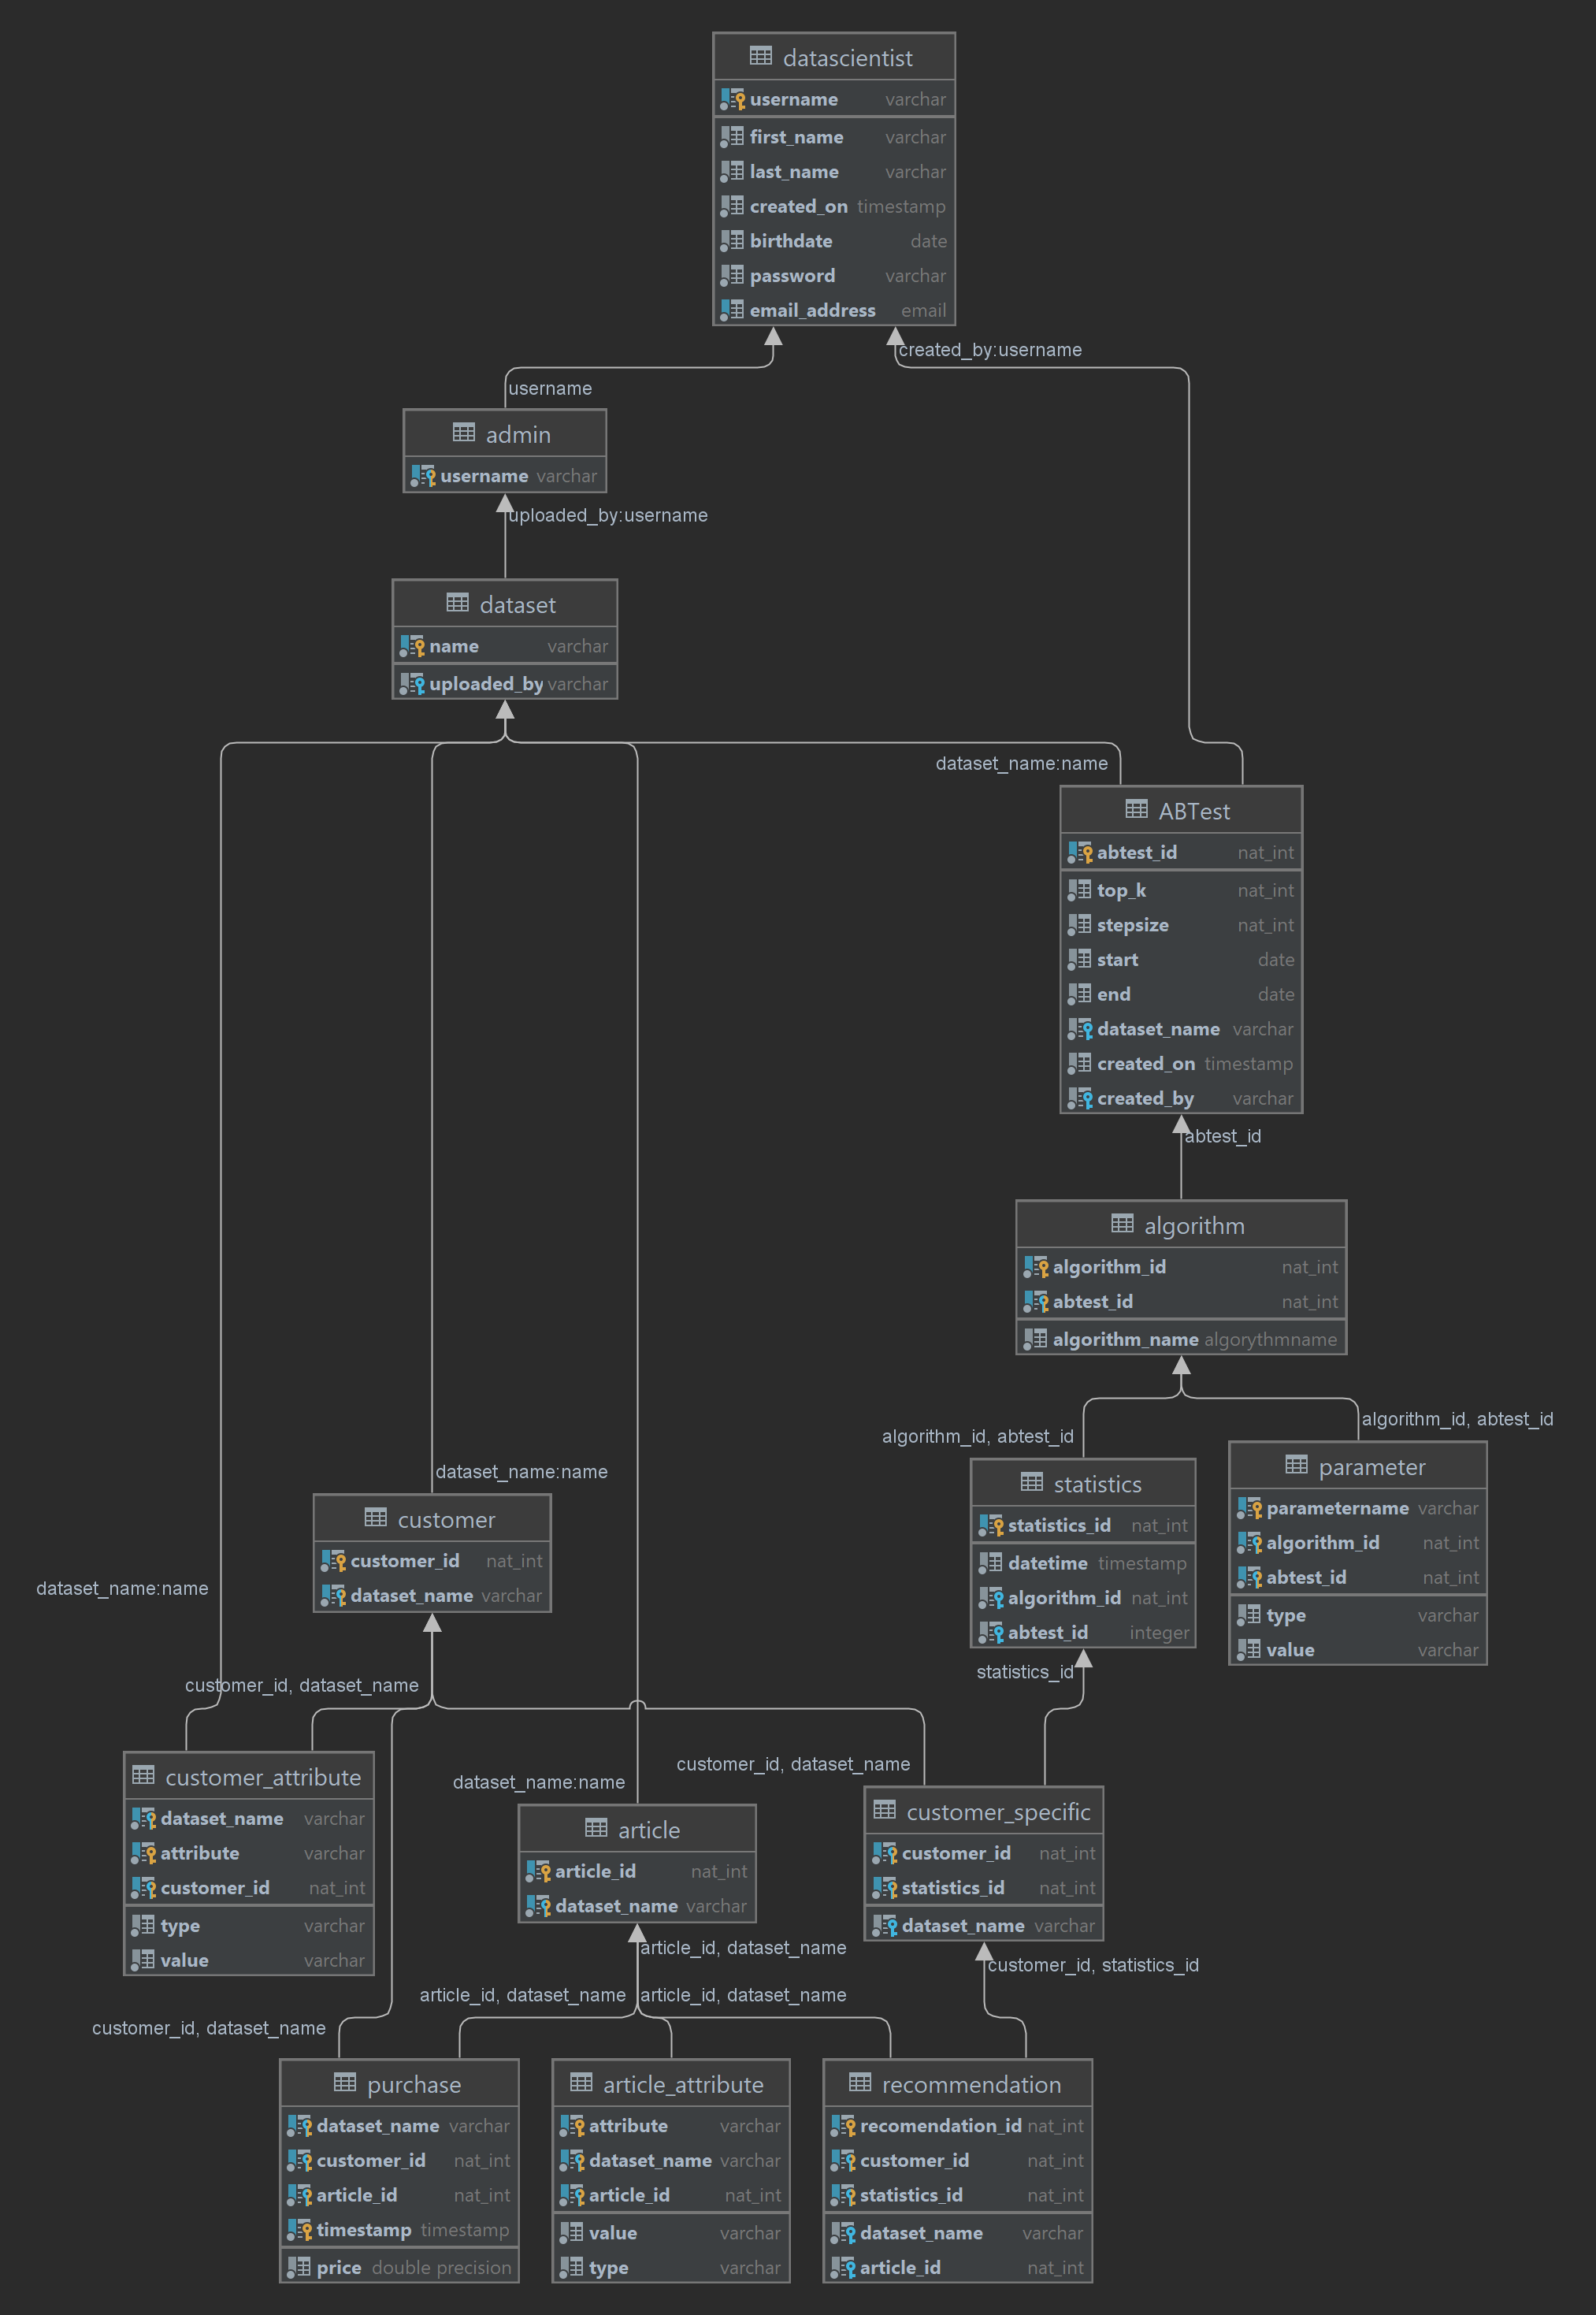
\includegraphics[height=600px]{FullDiagraph.png}
\end{center}
\restoregeometry     
	\pagebreak
	\section{Users}
	\subsection{datascientist}
	First we have the datascientist which all have a unique username (PK). They can log in onto the site and create ABTests, view their history and look at the datasets. Every user has a first and last name, creation date of the account, birth-date and password and unique email-address. 

	\subsection{Admin}
	An admin has a 'isa' relationship with a datascientist. An admin s the only one who can upload datasets of purchases, customers and articles. Admin is connected through a foreign key to datascientist, which is also its only field and its primary key.
		\begin{center}
		  		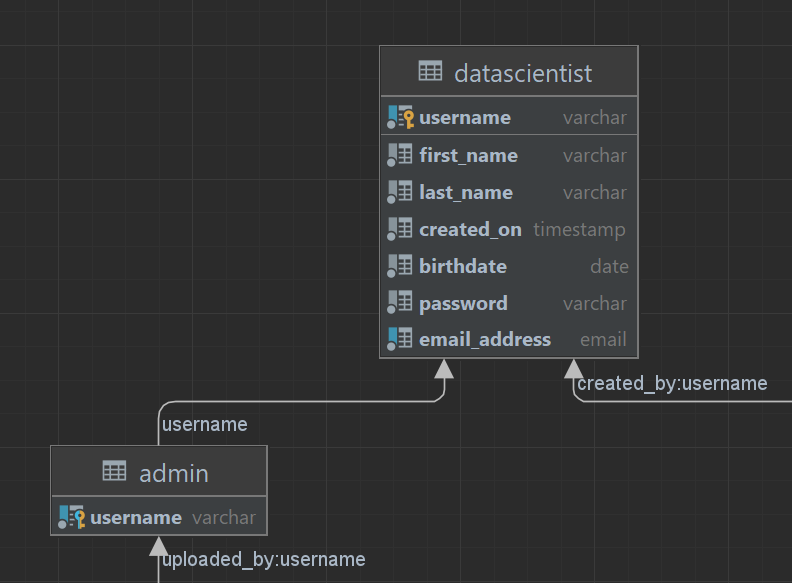
\includegraphics[height={200px},width=\textwidth,keepaspectratio]{Users.png}
		  		\includegraphics[height={200px},width=\textwidth,keepaspectratio]{Users.postgresql.png}
	\end{center}
	\pagebreak
	\section{Dataset}
	A dataset has a dataset-name as primary key. It is connected to an admin through a foreign key "uploaded-by" as only admins can upload such a set.
	\begin{center}
		  		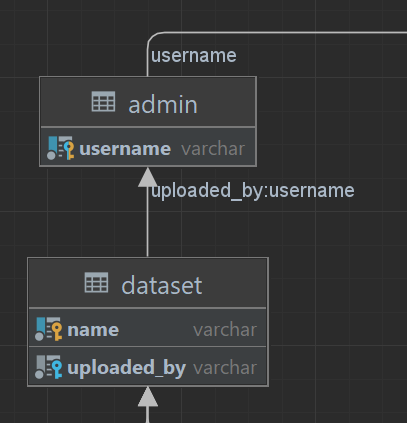
\includegraphics[height={200px},width=\textwidth,keepaspectratio]{Dataset.png}
		  		\includegraphics[height={200px},width=\textwidth,keepaspectratio]{Dataset.postgresql.png}
	\end{center}
	\pagebreak
	\subsection{Customers}
	A customer has unique\_customer\_id as primary key, this is unique through the whole database, aside of that it also has a secondary key namely a composed of a dataset-name (foreign key to dataset) and a customer-id to differentiate between customers in a given dataset.
	\subsubsection{Customer-Attribute}	
	Customer Attribute is where we store the actual (dynamic) data of a customer. It is a weak entity of customer and therefore contains a foreign key to a customer (customer-id, dataset-name). On top of this foreign key, the "attribute" is added which is the name of the field/attribute. So the final primary/composite key is (customer-id, dataset-name, attribute). It has a type and a value so it can be used as intended.
	
	\begin{center}
		  		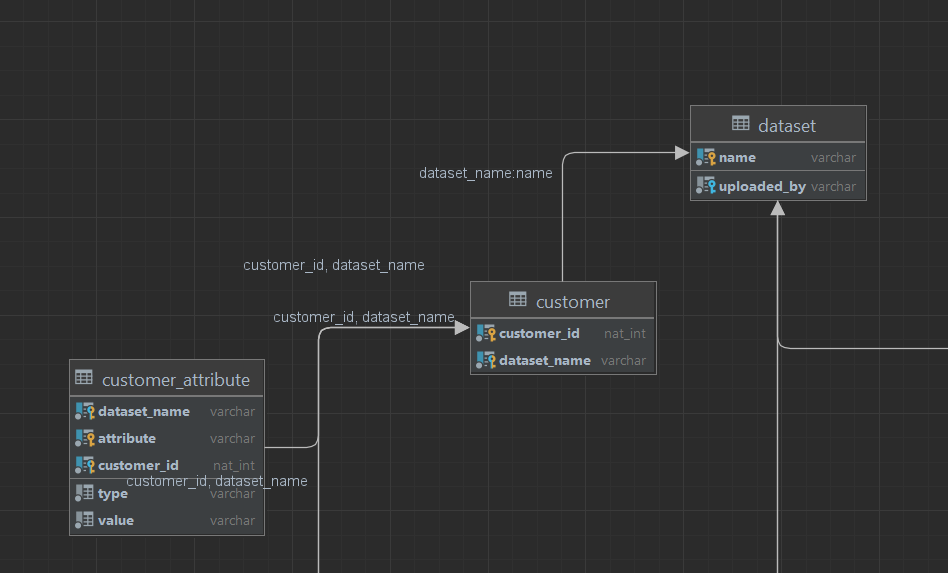
\includegraphics[height={200px},width=\textwidth,keepaspectratio]{Customer.png}
		  		\includegraphics[height={200px},width=\textwidth,keepaspectratio]{Customer.postgresql.png}
		  		\includegraphics[height={200px},width=\textwidth,keepaspectratio]{Customer_attribute.postgresql.png}
	\end{center}
	\pagebreak
	\subsection{Articles}
		An Article has a unique article id throughout the dataset as primary key. It also has a secondary key namely a composed of a dataset-name (foreign key to dataset) and an article-id to differentiate between articles in a given dataset = PK[dataset-name, article-id].
		\subsubsection{Article-Attribute}
			Article Attribute is where we store the actual (dynamic) data of an article. It is a weak entity of article and therefore contains a foreign key to an article (article-id, dataset-name). On top of this foreign key, the "attribute" is added which is the name of the field/attribute. So the final primary/composite key is (article-id, dataset-name, attribute). It has a type and a value so it can be used as intended.
	\begin{center}
		  		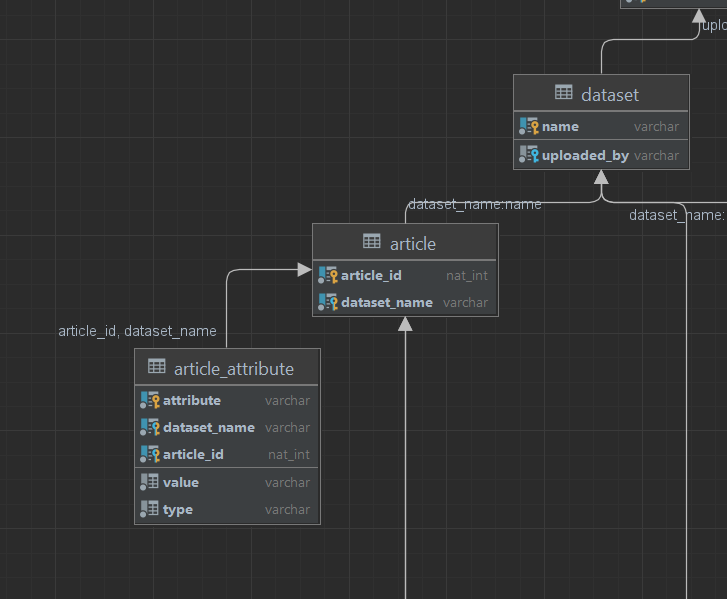
\includegraphics[height={200px},width=\textwidth,keepaspectratio]{Article.png}
	\end{center}
	\pagebreak	
	\subsection{Purchases}
	A purchase is defined by a person with "customer-id" buying an article with "article-id" belonging to the same dataset on "timestamp" for the price "price". Therefore the primary key of a purchase is (article-id,customer-id, dataset-name, timestamp). The price at the time of purchase is kept in an extra field. It references to customer(customer-id, dataset-name ) and article(article-id, dataset-name ), with the same dataset-name in both references.
		\begin{center}
		  		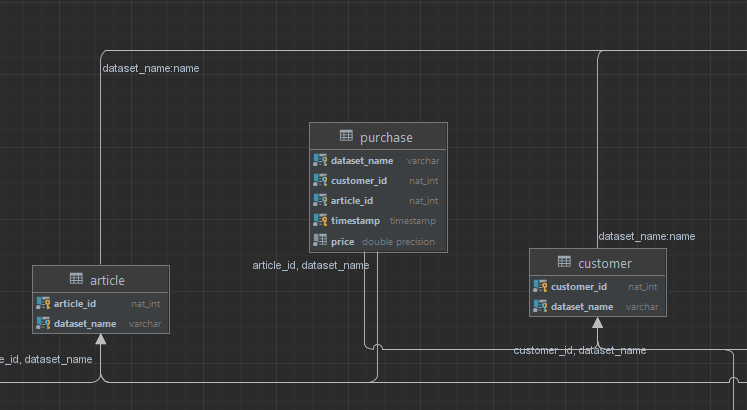
\includegraphics[height={200px},width=\textwidth,keepaspectratio,width=\textwidth,keepaspectratio ]{Purchase.png}
	\end{center}
	\pagebreak	
	\section{ABTest}		
	An abtest has a unique id [PK], It contains the test-wide parameters namely top-k, stepsize,start,end and dataset-name which references dataset(dataset-name). Its creator is kept in "uploaded-by" which references a datascientist. And its creation time is also kept which defaults to now().
			\begin{center}
		  		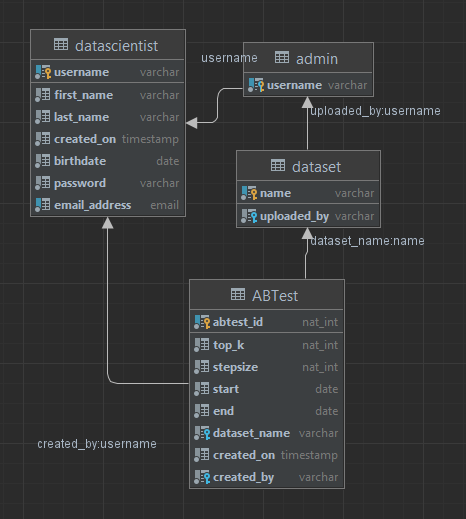
\includegraphics[width={250px}]{ABTest.png}
	\end{center}
	
	\subsection{Algorithm} An algorithm itself has an id as primary key and belongs to an abtest(abtest-id). It also contains the type of the algorithm (this is so that we can identify which exact algorithm we have to execute). We can make multiple algorithms and link them to the same ABTest.
\begin{center}

		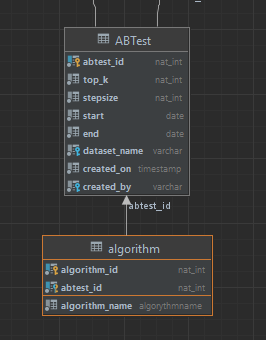
\includegraphics[height={200px},width=\textwidth,keepaspectratio]{Algorithm.png}
		\includegraphics[height={200px},width=\textwidth,keepaspectratio]{Algorithm.postgresql.png}
	
\end{center}			
	\subsubsection{Parameter} Parameter contains the name and value of a parameter that belongs to the algorithm. A parameter is a weak entity of an algorithm. The name of the parameter is unique in a given algorithm and thus the PK(parametername,algorithm-id,ABTest-id) where (algorithm-id,ABTest-id) references an algorithm.
\begin{center}
		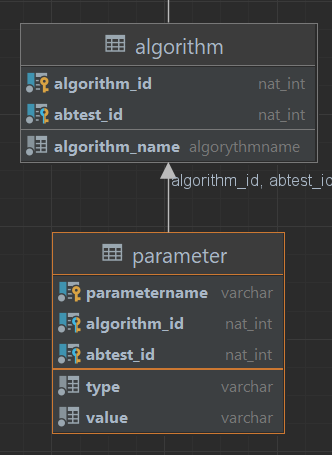
\includegraphics[height={200px},width=\textwidth,keepaspectratio]{Parameter.png}
		\includegraphics[height={200px},width=\textwidth,keepaspectratio]{Parameter.postgresql.png}
		
\end{center}
	\subsection{Statistics}
	Statistics has a primary key in the form of "statistics-id" but a secondary key (abtest-id, algorithm-id, datetime) is also present. Statistics holds the data that is fetched on a given date. One entity of statistics is kept per stepsize.
	\begin{center}
	
		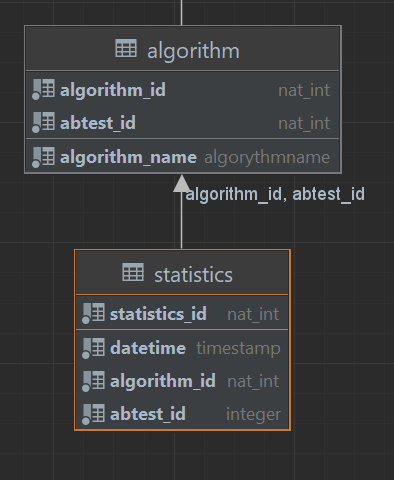
\includegraphics[height={200px},width=\textwidth,keepaspectratio]{Statistics.png}
		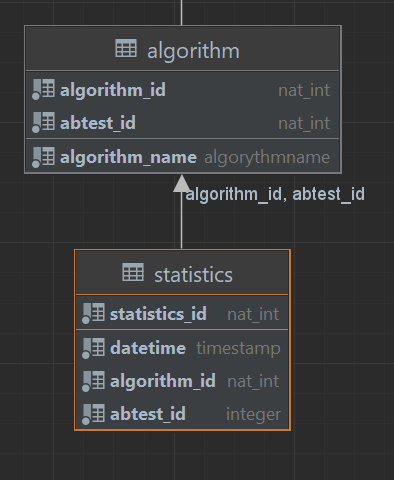
\includegraphics[height={200px},width=\textwidth,keepaspectratio]{Statistics.postgresql}
	\end{center}
\subsubsection{Dynamic-Stepsize-Variable}
	Dynamic-Stepsize-Variable allows for storing variables on every stepsize, therefore it has a foreign key to statistics. The PK = [statistics,parameter-name]. Aside of that it has the value that we want to store in parameter-value.
	\begin{center}
		\includegraphics[height={200px},width=\textwidth,keepaspectratio]{DSV.postgresql.png}
	
	\end{center}

\subsubsection{Customer-Specific-Statistics}
	Here we keep an entry with customer specific data for every customer that has been active (bought something) on the date present in statistics. Customer-specific is a weak entity with of statistics with PK(statistics-id,unique=customer-id). It basically links statistics with customer without copying the fields of statistics mindlessly.
		\begin{center}
		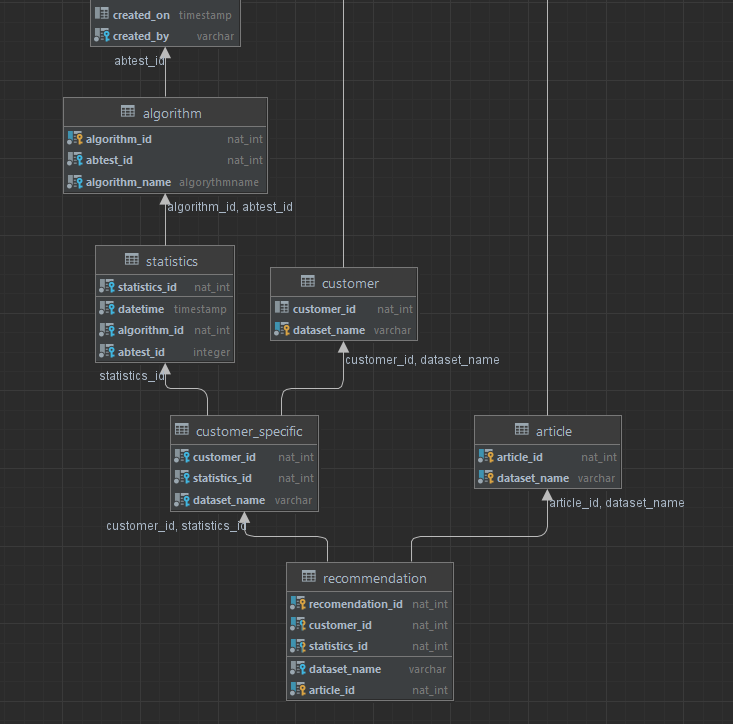
\includegraphics[height={200px},width=\textwidth,keepaspectratio]{Customer-Specific.png}
		\includegraphics[height={200px},width=\textwidth,keepaspectratio]{Customer_attribute.postgresql.png}
\end{center}		
	
	\subsubsection{recommendation}
	A recommendation entity is kept for every recommendation, this table links the customer-specific statistics with the recommendation-id Which goes up to k-1 in a top-k scenario. It is a weak entity of customer-specific. Its PK = [recommendation-id, unique-customer-id, statistics-id]. It has a foreign key to its stronger entity customer-specific and unique-article-id. It can be traced back to the "recommendation-id"th recommendation of customer "unique-customer-id" at (next are linked via statistics-id) "datetime" from algorithm "algorithm-id" in abtest "abtest-id". And even further to dataset and parameters if needed.  
	\begin{center}

		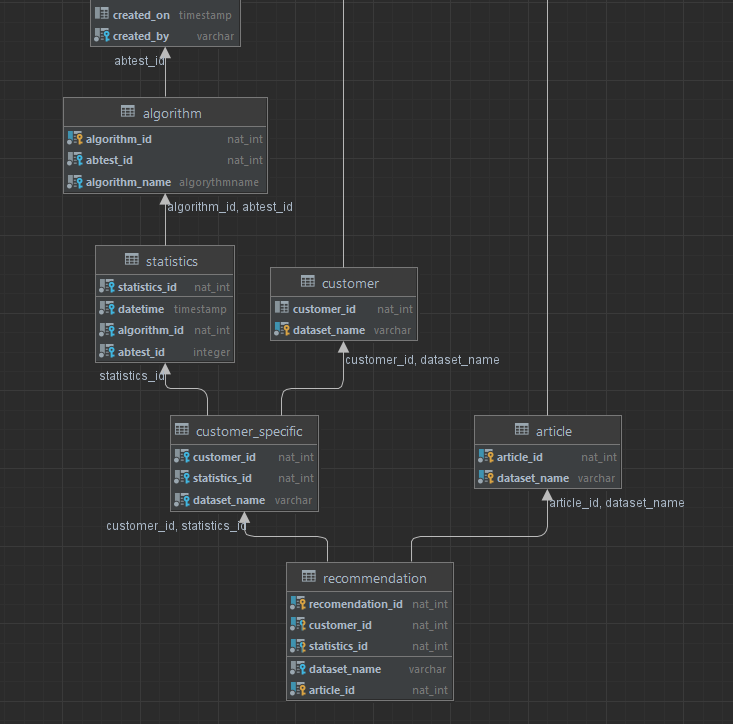
\includegraphics[height={300px}]{Customer-Specific.png}
		\includegraphics[height={200px},width=\textwidth,keepaspectratio]{Recommendation.postgresql.png}

\end{center}		
\section{Metrics}
Datetime is available in the table of statistics and all dependencies so it is accessible and can be used to chose a window size. 
\subsection{Purchases over time}
Can be done using a simple query where we count the purchases made within a single day for every day in the ABTest, we query for dataset\_name, start\_start and end\_date. \\
SELECT bought\_on,COUNT(unique\_article\_id)\\
FROM purchase NATURAL JOIN article\\
WHERE bought\_on between '{start}' and '{end}' and dataset\_name = '{dataset\_name}'  \\
            group by bought\_on;\\

\subsection{Unique Active Users Over Time}
Can be done using a simple query very similar to Purchases over time: \\
\begin{verbatim}
	SELECT bought_on,COUNT(DISTINCT(unique_customer_id))
	FROM purchase NATURAL JOIN customer
	WHERE bought_on between '{start}' and '{end}' and
		dataset_name = '{dataset_name}'
	group by bought_on;
\end{verbatim}
           
\subsection{Click Through Rate (CTR)}
\begin{spverbatim}
We know all the purchases that have been made and all the top-k list so we can figure out the click through rate. We calculate the ctr per day beforehand and store it into dynamic_stepsize_variable. Now we can fetch it over time with the following query:
SELECT date_of, algorithm_id,parameter_value, algorithm_name
FROM statistics 
	NATURAL JOIN dynamic_stepsize_var 
	NATURAL JOIN named_algorithm 
	NATURAL JOIN ab_test 
	WHERE abtest_id = {abtest_id} 
	AND parameter_name = 'CTR' 
	ORDER BY date_of;
\end{spverbatim}
\subsection{Attributions} 
\begin{spverbatim}
We can take an intersection of purchases and recommendations, we can see divide the count of purchases with this intersection over a period of 7 or 30 days.

Firstly we find the intersection, and count the times it was recommended. We filter on distinct articles as two recommendations on the same article in the past days only results attribution point to the algorithm.algorithm_id on bought_on for customer recommendation.unique_customer_id, the interval can be entered dynamically in this query (7 days in this case). We would only have to run this once per ABTest.


\end{spverbatim}
		\begin{center}
		  		\includegraphics[height={200px},width=\textwidth,keepaspectratio]{AttributionsView.png}
		  		query
		  		\includegraphics[height={200px},width=\textwidth,keepaspectratio]{Attributions_Example.png}
		  		Example of the query-result
	\end{center}
\begin{spverbatim}
The query is encapsulated in a materialized view for two reasons. Firstly we can index on it and use it to calculate our average attributions rate for one user over a period or for all users over the time (thus per day). Secondly we can also speed up all of the following queries by pre calculating the most intensive part.


\end{spverbatim}
\subsection{Attribution Rate (AR@D)} 
Next the sum of the attribution count for a customer over a period can be taken and divided by the number of purchases the customer has made in the same period, this is the attribution rate.


		\begin{center}
		  		\includegraphics[height={200px},width=\textwidth,keepaspectratio,width=\textwidth,keepaspectratio]{AttributionsRate.png}
		  		query
	\end{center}
\subsection{Average Revenue Per User (ARPU@D)}
At last, total revenue attributed to the algorithm for the user over an interval can be easily calculated.

		\begin{center}
		  		\includegraphics[height={200px},width=\textwidth,keepaspectratio,width=\textwidth,keepaspectratio]{ARPU.png}
		  		query
\end{center}
\end{document}
